% Options for packages loaded elsewhere
\PassOptionsToPackage{unicode}{hyperref}
\PassOptionsToPackage{hyphens}{url}
\PassOptionsToPackage{dvipsnames,svgnames,x11names}{xcolor}
%
\documentclass[
  letterpaper,
  DIV=11,
  numbers=noendperiod]{scrartcl}

\usepackage{amsmath,amssymb}
\usepackage{iftex}
\ifPDFTeX
  \usepackage[T1]{fontenc}
  \usepackage[utf8]{inputenc}
  \usepackage{textcomp} % provide euro and other symbols
\else % if luatex or xetex
  \usepackage{unicode-math}
  \defaultfontfeatures{Scale=MatchLowercase}
  \defaultfontfeatures[\rmfamily]{Ligatures=TeX,Scale=1}
\fi
\usepackage{lmodern}
\ifPDFTeX\else  
    % xetex/luatex font selection
\fi
% Use upquote if available, for straight quotes in verbatim environments
\IfFileExists{upquote.sty}{\usepackage{upquote}}{}
\IfFileExists{microtype.sty}{% use microtype if available
  \usepackage[]{microtype}
  \UseMicrotypeSet[protrusion]{basicmath} % disable protrusion for tt fonts
}{}
\makeatletter
\@ifundefined{KOMAClassName}{% if non-KOMA class
  \IfFileExists{parskip.sty}{%
    \usepackage{parskip}
  }{% else
    \setlength{\parindent}{0pt}
    \setlength{\parskip}{6pt plus 2pt minus 1pt}}
}{% if KOMA class
  \KOMAoptions{parskip=half}}
\makeatother
\usepackage{xcolor}
\setlength{\emergencystretch}{3em} % prevent overfull lines
\setcounter{secnumdepth}{-\maxdimen} % remove section numbering
% Make \paragraph and \subparagraph free-standing
\makeatletter
\ifx\paragraph\undefined\else
  \let\oldparagraph\paragraph
  \renewcommand{\paragraph}{
    \@ifstar
      \xxxParagraphStar
      \xxxParagraphNoStar
  }
  \newcommand{\xxxParagraphStar}[1]{\oldparagraph*{#1}\mbox{}}
  \newcommand{\xxxParagraphNoStar}[1]{\oldparagraph{#1}\mbox{}}
\fi
\ifx\subparagraph\undefined\else
  \let\oldsubparagraph\subparagraph
  \renewcommand{\subparagraph}{
    \@ifstar
      \xxxSubParagraphStar
      \xxxSubParagraphNoStar
  }
  \newcommand{\xxxSubParagraphStar}[1]{\oldsubparagraph*{#1}\mbox{}}
  \newcommand{\xxxSubParagraphNoStar}[1]{\oldsubparagraph{#1}\mbox{}}
\fi
\makeatother


\providecommand{\tightlist}{%
  \setlength{\itemsep}{0pt}\setlength{\parskip}{0pt}}\usepackage{longtable,booktabs,array}
\usepackage{calc} % for calculating minipage widths
% Correct order of tables after \paragraph or \subparagraph
\usepackage{etoolbox}
\makeatletter
\patchcmd\longtable{\par}{\if@noskipsec\mbox{}\fi\par}{}{}
\makeatother
% Allow footnotes in longtable head/foot
\IfFileExists{footnotehyper.sty}{\usepackage{footnotehyper}}{\usepackage{footnote}}
\makesavenoteenv{longtable}
\usepackage{graphicx}
\makeatletter
\def\maxwidth{\ifdim\Gin@nat@width>\linewidth\linewidth\else\Gin@nat@width\fi}
\def\maxheight{\ifdim\Gin@nat@height>\textheight\textheight\else\Gin@nat@height\fi}
\makeatother
% Scale images if necessary, so that they will not overflow the page
% margins by default, and it is still possible to overwrite the defaults
% using explicit options in \includegraphics[width, height, ...]{}
\setkeys{Gin}{width=\maxwidth,height=\maxheight,keepaspectratio}
% Set default figure placement to htbp
\makeatletter
\def\fps@figure{htbp}
\makeatother
% definitions for citeproc citations
\NewDocumentCommand\citeproctext{}{}
\NewDocumentCommand\citeproc{mm}{%
  \begingroup\def\citeproctext{#2}\cite{#1}\endgroup}
\makeatletter
 % allow citations to break across lines
 \let\@cite@ofmt\@firstofone
 % avoid brackets around text for \cite:
 \def\@biblabel#1{}
 \def\@cite#1#2{{#1\if@tempswa , #2\fi}}
\makeatother
\newlength{\cslhangindent}
\setlength{\cslhangindent}{1.5em}
\newlength{\csllabelwidth}
\setlength{\csllabelwidth}{3em}
\newenvironment{CSLReferences}[2] % #1 hanging-indent, #2 entry-spacing
 {\begin{list}{}{%
  \setlength{\itemindent}{0pt}
  \setlength{\leftmargin}{0pt}
  \setlength{\parsep}{0pt}
  % turn on hanging indent if param 1 is 1
  \ifodd #1
   \setlength{\leftmargin}{\cslhangindent}
   \setlength{\itemindent}{-1\cslhangindent}
  \fi
  % set entry spacing
  \setlength{\itemsep}{#2\baselineskip}}}
 {\end{list}}
\usepackage{calc}
\newcommand{\CSLBlock}[1]{\hfill\break\parbox[t]{\linewidth}{\strut\ignorespaces#1\strut}}
\newcommand{\CSLLeftMargin}[1]{\parbox[t]{\csllabelwidth}{\strut#1\strut}}
\newcommand{\CSLRightInline}[1]{\parbox[t]{\linewidth - \csllabelwidth}{\strut#1\strut}}
\newcommand{\CSLIndent}[1]{\hspace{\cslhangindent}#1}

\KOMAoption{captions}{tableheading}
\makeatletter
\@ifpackageloaded{caption}{}{\usepackage{caption}}
\AtBeginDocument{%
\ifdefined\contentsname
  \renewcommand*\contentsname{Table of contents}
\else
  \newcommand\contentsname{Table of contents}
\fi
\ifdefined\listfigurename
  \renewcommand*\listfigurename{List of Figures}
\else
  \newcommand\listfigurename{List of Figures}
\fi
\ifdefined\listtablename
  \renewcommand*\listtablename{List of Tables}
\else
  \newcommand\listtablename{List of Tables}
\fi
\ifdefined\figurename
  \renewcommand*\figurename{Figure}
\else
  \newcommand\figurename{Figure}
\fi
\ifdefined\tablename
  \renewcommand*\tablename{Table}
\else
  \newcommand\tablename{Table}
\fi
}
\@ifpackageloaded{float}{}{\usepackage{float}}
\floatstyle{ruled}
\@ifundefined{c@chapter}{\newfloat{codelisting}{h}{lop}}{\newfloat{codelisting}{h}{lop}[chapter]}
\floatname{codelisting}{Listing}
\newcommand*\listoflistings{\listof{codelisting}{List of Listings}}
\makeatother
\makeatletter
\makeatother
\makeatletter
\@ifpackageloaded{caption}{}{\usepackage{caption}}
\@ifpackageloaded{subcaption}{}{\usepackage{subcaption}}
\makeatother

\ifLuaTeX
  \usepackage{selnolig}  % disable illegal ligatures
\fi
\usepackage{bookmark}

\IfFileExists{xurl.sty}{\usepackage{xurl}}{} % add URL line breaks if available
\urlstyle{same} % disable monospaced font for URLs
\hypersetup{
  colorlinks=true,
  linkcolor={blue},
  filecolor={Maroon},
  citecolor={Blue},
  urlcolor={Blue},
  pdfcreator={LaTeX via pandoc}}


\author{}
\date{}

\begin{document}


\section{Philosophy of Teaching and
Learning}\label{philosophy-of-teaching-and-learning}

In my research and practice of teaching and learning in higher
education, I ground my work in three broad principles related to
\emph{who learners are}, \emph{what teachers do}, and \emph{how teachers
know what learners know}.

\subsection{Who Learners Are}\label{who-learners-are}

\begin{quote}
Those who seek to learn to improve themselves and the world around them
have inherent dignity and value.
\end{quote}

This principle is expanded in the 5 Rs of Indigenous education (Tessaro
et al. 2018): respect, responsibility, relevance, reciprocity, and
relationships. The 5 Rs serve as a set of values grounded in the
inherent value of all people and the importance of intentional work to
foreground the perspectives of equity-deserving groups. When diversity,
equity, and inclusion are prioritized and co-created, the entire
community of learners benefits from working in an environment where it
is safe to be different or wrong. The ultimate goal of education is to
empower learners to fully realize \emph{their} purpose and to flourish
in \emph{their} efforts to improve the world around \emph{them}.

This principle is reflected in the structure of my courses where
learners are always able to make meaningful choices about how their
learning will be demonstrated. For example, assignments are always
grounded in the course learning outcomes, and they require learners to
apply the concepts of the course to their own context. It is the learner
who determines relevance, and it is through the relationships developed
in the context of the course community that relevant learning is
expressed. Respect and reciprocity are demonstrated in the process of
co-creating a community of inquiry where all members share the
responsibility for the safety and well-being of others. The key to
making this all happen is that I host assessment conversations with
learners where we meet to discuss their work and come to a mutually
agreeable assessment of the quality of their work in light of the course
outcomes.

One learner in my class reflected on their experience during LDRS 663 in
their final paper (some details are omitted for anonymity):

\begin{quote}
Reflecting on these experiences, I've come to realize that
transformational learning through coaching and facilitation is not
simply a collection of tools; it is a deeply transformative mindset
rooted in empathy, openness, and a commitment to critically engaging
with deeply held beliefs. This mindset has profoundly reshaped my
\ldots{} identity, broadening my understanding of what it means to lead
a \ldots{} community. It challenges the notion of \ldots{} authority as
merely instructive, moving it instead toward a collaborative, relational
approach that invites people into a shared journey of growth and
exploration. Through this lens, my purpose has evolved into guiding our
{[}community{]} toward a new understanding of inclusivity---not as a
trend, but as an essential \ldots{} value grounded in love, curiosity,
and respect for diverse perspectives.
\end{quote}

\subsection{What Teachers Do}\label{what-teachers-do}

\begin{quote}
Learning is idealized as a cognitive apprenticeship which supports the
process of sense-making in the context of complex ideas.
\end{quote}

We know from Bloom (1984) that the most profound learning experiences
occur in the context of sustained discourse between a learner (or maybe
two or three) and an instructor (who can sometimes be a peer or other
interested observer). This sense-making process must include the learner
actively drawing connections between ideas and drawing conclusions that
are relevant to their own contexts. Sense-making is often a difficult
and tentative process, so it is incumbent on the instructor to allow
learners to do the work of learning and to recognize that not all
learners will achieve at the same pace. Learners exercise autonomy and
agency when they are encouraged to exercise evaluative judgement (Tai et
al. 2018) through the comparison of their own work to the work of both
novice and expert others and to the intended learning outcome. The task
of assessment is a similar process of the instructor making sense of
what the learner has demonstrated in their process and the products of
their work.

This principle is realized in my online courses in how I structure
discourse, or the conversation around course concepts. Learners are
required to demonstrate their process of coming to understand a topic or
task, not only submit a final product. A `discussion forum', which may
use various platforms such as blogs or social media, in any of my
courses is considered to be required, but not graded. The discussion
forum is not graded because I want my learners to be free to express
tentative or controversial ideas without fear of losing marks. Much like
conversations inside the four walls of a brick-and-mortar classroom,
which are not graded for accuracy, conversations in an online forum
should be considered as works-in-progress as learners make sense of
concepts and ideas. For graded assignments, learners are required to
submit their working documents in addition to the final, polished
version.

An example is this anonymized exerpt from a group project final
submission.

\begin{figure}[H]

{\centering 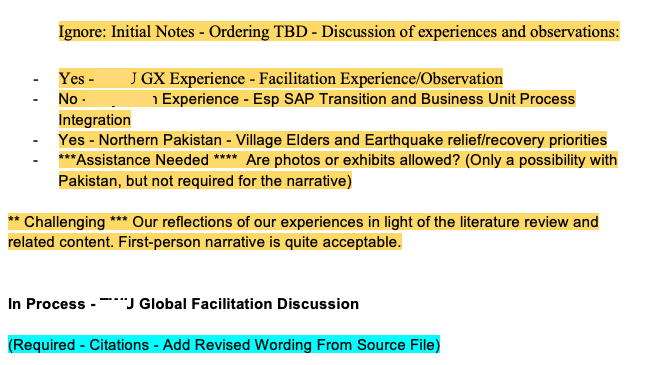
\includegraphics{assets/screenshot-sample-doc.png}

}

\caption{Screenshot of a portion of a MS Word document showing the
process of discussing the task.}

\end{figure}%

Assessment conversations are a key component of allowing me to come to
understand what the learner knows or can do. By having a conversation
that includes talking about their working docs and the final product, I
can get a clearer picture of the learner's ability, I can ask clarifying
questions in the moment, and the learner can provide valuable context to
their work.

\subsection{How Teachers Know What Learners
Know}\label{how-teachers-know-what-learners-know}

\begin{quote}
If there is an end, it is when the teacher has become unnecessary.
\end{quote}

Coming to know something (learning) is a result of what we do. When
learners strive for a cognitive goal, they iterate based on their past
knowledge combined with feedback they receive regarding their
performance in relation to the goal (Carless 2019; Hattie and Timperley
2007). Consequently, learning is inextricably tied to the process of
assessing learning. Traditional models of learning require significant
time and effort on the part of instructors who are the primary source of
feedback in the process. Contrary to that, when a learner is able to
generate their own feedback on performance, they are no longer
completely reliant on the instructor and can sustain and direct their
own learning (Boud and Soler 2016). I believe this should become the
primary and overarching goal of higher education institutions, to
produce self-sustaining learners who work and live in communities of
inquiy for the good of the world.

An example of how this is realized in my courses is that learners are
free to choose their domains of inquiry in alignment with the intended
outcomes of the course. One of the outcomes in EDCI 335 is

\begin{quote}
Identify and evaluate various digital, networked, and open technologies
and understand how they impact the learners and the learning process
\end{quote}

Learners have meaningful options when it comes to meeting this
objective. They can demonstrate their knowledge by creating a short
learning experience using a Notion site where participants are led
through a lesson in Gender and Mental Health, as below:

\begin{figure}[H]

{\centering 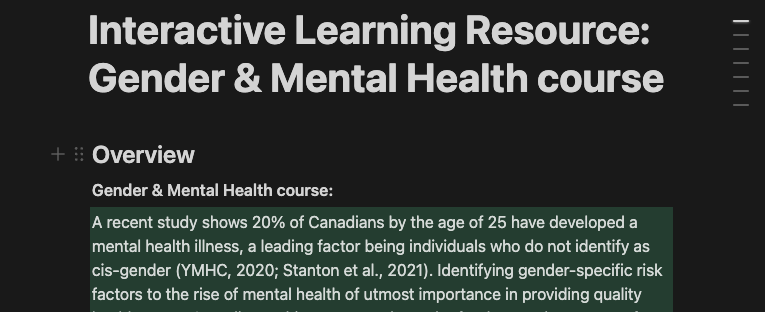
\includegraphics{assets/ilr-notion.png}

}

\caption{Screenshot of a learner-created lesson on Gender and Mental
Health using Notion as the platform.}

\end{figure}%

Or they may use Google Docs to teach others about the concept of Public
Goods in economics.

\begin{figure}[H]

{\centering 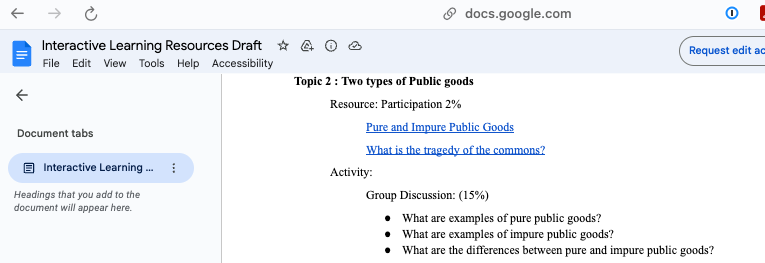
\includegraphics{assets/ILR-gdocs.png}

}

\caption{Screenshot of a learner-created lesson on Public Goods using
Google Docs as the platform.}

\end{figure}%

By encouraging learners to customize their outputs and review each
others' work, they are allowed to engage in work that is more relevant
to their own lives, and more likely to be able to sustain their learning
after my course has completed.

The most effective process of me coming to know what the learner knows
is to schedule 10-15 minute synchronous assessment conversations with
learners where they present their work. I thus have the opportunity in
the moment to probe their thinking about their work and to make a
determination of the authenticity of their performance.

In summary, I believe that all learners have inherent rights and
dignity, that teaching and learning is a relationship best described as
a cognitive apprenticeship, and that meaningful work and conversations
are the best ways to certify that learning has occured.

\section*{References}\label{references}
\addcontentsline{toc}{section}{References}

\phantomsection\label{refs}
\begin{CSLReferences}{1}{0}
\bibitem[\citeproctext]{ref-bloom1984}
Bloom, Benjamin. 1984. {``The 2 Sigma Problem: The Search for Methods of
Group Instruction as Effective as One-to-One Tutoring.''}
\emph{Educational Researcher} 13: 4--16.

\bibitem[\citeproctext]{ref-boud2016}
Boud, David, and Rebeca Soler. 2016. {``Sustainable Assessment
Revisited.''} \emph{Assessment \& Evaluation in Higher Education} 41
(3): 400--413. \url{https://doi.org/10.1080/02602938.2015.1018133}.

\bibitem[\citeproctext]{ref-carless2019}
Carless, David. 2019. {``Feedback Loops and the Longer-Term: Towards
Feedback Spirals.''} \emph{Assessment \& Evaluation in Higher Education}
44 (5): 705--14. \url{https://doi.org/10.1080/02602938.2018.1531108}.

\bibitem[\citeproctext]{ref-hattie2007}
Hattie, John, and Helen Timperley. 2007. {``The Power of Feedback.''}
\emph{Review of Educational Research} 77 (March): 81--112.
\url{https://doi.org/10.3102/003465430298487}.

\bibitem[\citeproctext]{ref-tai2018}
Tai, Joanna, Rola Ajjawi, David Boud, Phillip Dawson, and Ernesto
Panadero. 2018. {``Developing Evaluative Judgement: Enabling Students to
Make Decisions about the Quality of Work.''} \emph{Higher Education} 76
(3): 467--81. \url{https://doi.org/10.1007/s10734-017-0220-3}.

\bibitem[\citeproctext]{ref-tessaro2018}
Tessaro, Danielle, Jean-Paul Restoule, Patricia Gaviria, Joseph Flessa,
Carlana Lindeman, and Coleen Scully-Stewart. 2018. {``The Five r's for
Indigenizing Online Learning: A Case Study of the First Nations Schools'
Principals Course.''} \emph{Canadian Journal of Native Education} 40
(1): 125--43.
\url{https://www.researchgate.net/publication/328289320_The_Five_R\%27s_for_Indigenizing_Online_Learning_A_Case_Study_of_the_First_Nations_Schools\%27_Principals_Course}.

\end{CSLReferences}




\end{document}
